\section{Referencial Teórico}\label{sec:referencial-teorico}


Nesta Seção os principais conceitos relacionados a este trabalho são apresentados, fornecendo subsídios para o desenvolvimento do projeto proposto. A subseção \ref{sec:contexto-geral} apresenta o contexto no qual o projeto está inserido. As subseções \ref{sec:comp-movel},\ref{sec:comp-prevasiva} e \ref{sec:comp-ubiqua} apresentam a distinção entre os conceito de Computação Móvel, Computação Pervasiva e Computação Ubíqua. Por fim, na subseção \ref{sec:topico-3} é abordado o assunto cccc.

\subsection{Contexto Geral}\label{sec:contexto-geral}

O termo Computação Ubíqua foi definido pela primeira vez por Mark Weiser \cite{weiser1991} no final dos anos 80. Nesta época, Weiser previa um aumento das funcionalidades e da disponibilidade de serviços de computação para os usuários finais e, por outro lado, ele previa uma diminuição da visibilidade destes serviços. Para Weiser, a computação não seria exclusividade de um computador. Ele acreditava que no futuro existiriam diversos dispositivos diferentes conectados entre si. Em uma época que os usuários usavam PCs (Desktops) e para isso precisavam de conhecimento para operar um computador, Weiser apostou em um futuro onde foco dos usuários seria a tarefa em si, e não a ferramenta utilizada. Desta forma, eles usariam a computação sem perceber ou necessitar de conhecimentos técnicos específicos \cite{weiser1994world}.
					
O passar do tempo demonstrou que a aposta de Weiser foi acertada. Para Weiser \cite{weiser1997coming}, a evolução da computação passou por duas eras até chegar a Computação Ubíqua. A primeira delas foi denominada era do mainframe onde muitas pessoas compartilhavam um mesmo computador. A segunda era foi a do PC onde cada computador era usado por uma pessoa. Atualmente, a evolução dos sistemas de informação distribuídos, a ampliação das opções de tipos conexões a rede, a computação móvel e os diversos tipos de aplicações sobre dispositivos computacionais não convencionais, são apenas alguns dos exemplos que permitem afirmar: a Computação Ubíqua (a terceira era) já é uma realidade. A figura ~\ref{fig:era} mostra um gráfico com as eras da computação, segundo Mark Weiser.

\begin{figure}[ht]
\centering
    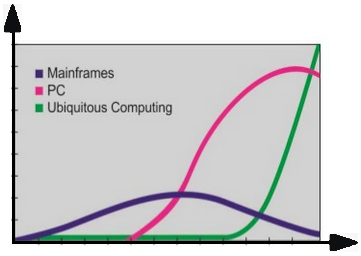
\includegraphics[width=0.4\textwidth,natwidth=610,natheight=642]{images/era.png}
    \caption{Eras da Computação}
    \label{fig:era}
\end{figure}

Termos como Computação Ubíqua, computação pervasiva, computação nomádica, computação invisível, computação móvel e outros tantos, têm sido usados muitas vezes como sinônimos, embora sejam diferentes conceitualmente e empreguem diferentes ideias de organização e gerenciamento dos serviços computacionais. Na medida em que cada área evolui, esses conceitos vão sendo melhor compreendidos e suas definições se tornam mais claras. Esta seção apresenta os principais conceitos necessários para compreensão da \textit{UbiComp} além de apresentar alguns exemplos de projetos encontrados na literatura. 


\subsection{Computação Móvel}\label{sec:comp-movel}
A computação móvel baseia-se na capacidade de um usuário carregar/mover (fisicamente) serviços computacionais para onde quer que ele se mova. Neste contexto, o computador torna-se um dispositivo sempre presente que expande a capacidade de um usuário utilizar os serviços que ele oferece, independentemente de sua localização. Combinada com a capacidade de acesso a rede, a computação móvel tem transformado a computação numa atividade que pode ser levada para praticamente qualquer local \cite{netodesenvolvimento}.
					
Uma importante limitação conceitual da computação móvel é que o modelo computacional utilizado na maioria das aplicações não muda enquanto os usuários se movem. Isto significa que um dispositivo não é capaz de obter informação sobre o contexto físico no qual a computação ocorre, e, como consequência, também não consegue se adequar ao novo contexto corretamente. Uma solução para acomodar a mudança de contexto seria passar aos usuários a responsabilidade de controlar e configurar manualmente uma aplicação/dispositivo na medida em que ele se movem. Contudo, esta solução não é bem aceita pela maioria dos usuários. Essa limitação foi uma das inspirações para a Computação Pervasiva. 

\subsection{Computação Pervasiva}\label{sec:comp-prevasiva}
O conceito de computação pervasiva implica que o computador está embarcado no ambiente de forma invisível para o usuário \cite{krumm2009}. Nessa concepção, o computador tem a capacidade de: i) obter informação do ambiente no qual ele está embarcado e ii) utilizá-la para construir, dinamicamente, modelos computacionais que permitem controlar, configurar e ajustar a aplicação para melhor atender as necessidades de um dispositivo ou usuário. Para que isso seja possível, o ponto fundamental é a capacidade dos computadores poderem agir de forma “inteligente” no ambiente no qual os usuários se movem. Esse ambiente é normalmente povoado por sensores e serviços computacionais. 

\subsection{Computação Ubíqua}\label{sec:comp-ubiqua}
Como pode ser visto na Figura~\ref{fig:ubiq}, a \textit{UbiComp} pode ser definida como uma área da computação posicionada entre a computação móvel e a computação pervasiva \cite{krumm2009,de2003computaccao}. A palavra Ubíquo é um adjetivo de origem no Latim (\textit{ubiquu}) que significa “aquilo está ao mesmo tempo em toda a parte”. A Computação Ubíqua beneficia-se dos avanços da computação móvel e da computação pervasiva e surge da necessidade de se integrar mobilidade com a funcionalidade da computação pervasiva. O termo Computação Ubíqua será usado aqui como uma junção da computação pervasiva e da computação móvel. A justificativa de se realizar uma diferenciação desses termos é que um dispositivo que está embutido em um ambiente, não necessariamente é móvel. 

\begin{figure}[h]
\centering
    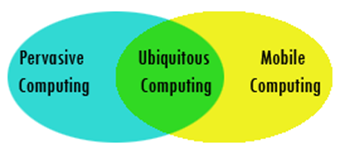
\includegraphics[width=0.4\textwidth,natwidth=610,natheight=642]{images/ubiq.png}
    \caption{Computação Ubíqua: interseção entre computação pervasiva e móvel}
    \label{fig:ubiq}
\end{figure}
				
Pesquisas na área de Computação Ubíqua abordam sobre as tecnologias e infra-estruturas que viabilizam a implantação de aplicações Ubíquas através de uma série de questões dentre elas:

 \begin{itemize}
   \item Como projetar \textit{hardwares} e sistemas operacionais para plataformas de sensores;
   \item Como permitir que dispositivos encontrem uns ao outros e utilizem seus serviços;
   \item Como permitir que sistemas envolvendo recursos limitados de processamento e energia funcionem.
 \end{itemize}
 
 Geralmente, as aplicações Ubíquas recebem dados de sensores, de outros dispositivos provedores de serviços, gerenciam ações de usuários, oferecem suporte à mobilidade e utilizam informações de contexto para execução de tarefas \cite{doesntfit}. Um sistema Ubíquo propriamente dito possui um conjunto de requisitos, peculiaridades e desafios que influenciam na concepção, implementação, implantação e avaliação de seu projeto \cite{krumm2009}. Estes são pontos fundamentais para \textit{UbiComp} e bem diferente daqueles usadas no desenvolvimento de sistemas para PCs. Dentre estes pontos, podemos citar como exemplo \cite{krumm2009}: 
 
 \begin{enumerate}
   \item Dispositivos de recursos limitados (\textit{Resource-Constrained Devices});	
   \item Ambientes de execução voláteis (\textit{Volatile Execution Environments});	
   \item Ambientes de execução heterogêneos (\textit{Heterogeneous Execution Environments});
   \item Ambientes de uso flutuantes (\textit{Fluctuating Usage Environments});
   \item Computação invisível (\textit{Invisible Computing});
   \item Segurança e privacidade (\textit{Security and Privacy}). 
 \end{enumerate}


São consideradas as principais propriedades da Computação Ubíqua \cite{lyytinen2002ubiquitous}:

 \begin{itemize}
   \item Integração física: Espaços inteligentes são definidos pela colaboração intensa entre elementos computacionais e componentes do mundo físico;
   \item Invisibilidade: Extingue-se a integração entre o homem e o computador e deixa-se que ambas entidades convivam em perfeita simbiose;
   \item Pró-atividade: É a capacidade do sistema antecipar a intenção do usuário;
   \item Sensibilidade ao contexto: O cenário de interação influencia nas interações;
   \item Interoperabilidade: Ambiente Ubíquos são compostos por dispositivos operacionais heterogêneos;
   \item Interoperabilidade Espontânea: É a possibilidade de integração dinâmica entre componentes móveis e a infraestrutura do sistema, sem a intervenção do usuário;
   \item Interfaces Naturais: Interações através de gestos, voz e olhares;
   \item Coordenação: Interações síncronas e assíncronas através de várias entidades computacionais podem ser realizadas a todo momento;
   \item Adaptação e tolerância a falhas: O sistema deve se adaptar automaticamente a falhas nos serviços disponíveis, na rede e nos dispositivos;
   \item Mobilidade: usuários, dispositivos e serviços podem mover-se dentro de um mesmo ambiente e entre ambientes distintos.
 \end{itemize}

\subsection{Internet das coisas(IoT)}\label{iot}

A Internet das Coisas (IoT) é um domínio multidisciplinar, que abrange um grande número de temas, desde questões puramente técnicas (por exemplo, protocolos de roteamento, consultas semânticas), a uma mistura de problemas técnicos e sociais (segurança, privacidade, usabilidade), bem como temas sociais e empresariais. As aplicações da Internet das coisas, existentes são potencialmente diversas. Vigilância da saúde ambiental e pessoal, monitoramento e controle de processos industriais, incluindo a agricultura, espaços inteligentes e cidades inteligentes são apenas alguns dos exemplos de aplicações da Internet das coisas \cite{krishnakumarframework}.
